\chapter{Architektur}
An dieser Stelle wird der Aufbau von Masterly Mate geschildert, welcher nicht
unmittelbar durch einen Anwender wahrgenommen wird.

\section{Erweiterbarkeit}
Bei der Konzeption wird insbesondere darauf geachtet, dass die Anwendung einfach
erweiterbar ist und den Ansprüchen vielseitiger Szenarien genügt.
So wird beispielsweise auf die Unterstützung von WBTs aus einem bestimmten
Autorenwerkzeug verzichtet. Viel mehr steht das Einbinden von SCORM auf dem
Plan. Darüber hinaus berücksichtigt das Klassenmodell (siehe Abschnitt
\ref{ref:classModel}) eine Many-to-Many Beziehung zwischen Themen und WBTs. So
ist gewährleistet, dass es allgemeine WBTs geben kann, die mehreren Themen
zugehörig sind.

\section{Aufbereiten des Dreyfus-Modells}\label{ref:dreyfusConcept} 
Für das Produkt der vorliegenden Studienarbeit wird das in Abschnitt
\ref{ref:dreyfus} erläuterte Dreyfus-Modell angepasst. So ergeben sich vier
fachliche Ränge. Hinzu kommen Ränge für Tutoren, welche einem Nutzer den fünften
Rang nach dem Dreyfus-Modell erreichen lässt. Hinzu kommt, dass der fachliche
Rang regelmäßig vom Nutzer bestätigt werden muss. Nach einem Jahr im selben Rang
wird der Nutzer aufgefordert einen Test zu absolvieren.
Besteht er den Test nicht, oder ignoriert er diesen, so fällt der Nutzer
automatisch um einen Rang. Da es keinen Rang unterhalb von "`novice"' gibt,
werden Nutzer automatisch gelöscht, die den Test für den untersten Rang nicht
bestehen. Diese Vorgehensweise wird so umgesetzt, da davon ausgegangen werden
kann, dass ein aktiver Nutzer innerhalb eines Jahres den nächst höheren Rang
erreicht. Weiterhin werden so inaktive und nicht interessierte Nutzer
automatisch entfernt, was in einer regen Gemeinschaft resultiert. Dem Problem
von Accounts, hinter dem kein aktiver Nutzer\footnote{sogenannten Zombies} mehr
steht, wird somit vorgebeugt.

\subsection{Fachlicher Rang}\label{ref:rankTopic}
Mit dem Durcharbeiten von WBTs kann ein Nutzer im fachlichen Rang aufsteigen.
Der Hintergrund ist, dass er mit korrekten Antworten im Prüfungsteil der WBTs
seine fachliche Kompetenz unter Beweis stellt. Demgegenüber werden bei falschen
Antworten im Quiz keine negativen Punkte angerechtnet. Je nachdem, wie gut ein
Test ausfällt, erhält er eine bestimmte Anzahl an Punkten. Abhängig vom Grad des
aktuellen fachlichen Rangs wird auch die notwendige Punktzahl für den nächsten
Rang erhöht. Der Aufbau folgt also analog einer Exponentialfunktion. Wie in
Abbildung \ref{ref:vertPunkt} zu sehen ist, benötigt man im Vergleich mit den
didaktischen Rängen im fachlichen Level mehr Punkte für den nächsten Rang. Im
Gegensatz dazu wird hier maximal der Experten-Rang erreicht. In der Abbildung
ist der Rang des Experten nicht zu sehen, da dieser das Erreichen der
notwendigen kompletten Punktzahl symbolisiert.

Selbstverständlich können weitere WBTs durchgearbeitet werden, diese bessern
jedoch nicht das Punktekonto für den fachlichen Rang auf. Dem Anwender ist
freigestellt, ob er sich nun, wo er Experte in einem Fachgebiet ist, einem
anderen Wissensgebiet widmet, um dort als Neuling von Vorn anzufangen.

\subsection{Ränge für Tutoren}\label{ref:rankTeach}
Als Tutor wird man von den Lernenden beurteilt, die man in einem gewissen
Fachgebiet unterstützt hat. Im Gegensatz zu den fachlichen Rängen sind die
didaktischen Ränge vom Fach unabhängig. Auch bleiben sie über alle fachlichen
Ränge hinweg erhalten. Ein weiterer Unterschied ist, dass man als Tutor nicht
Punkte, sondern Sterne sammelt. Jede gute Bewertung (daumen rauf) gibt einen
Schritt in Richtung weiteren Stern. Eine schlechte Bewertung (daumen runter)
stellt dazu einen direkten Gegensatz dar. Beide Bewertungsrichtungen verhalten
sich ausgeglichen und es kristallisieren sich Tutoren heraus, die fachliche
Inhalte für jedermann verständlich zu erklären wissen. Darüber hinaus kann ein
Tutor einen Stern verlieren, wenn er in einem Quartal keine Unterweisung
hällt. So ist gewährleistet, dass sich meisterliche Tutoren nicht auf ihren vier
Sternen "`ausruhen"'.

Meisterliche Tutoren verfügen auch über das Privileg eigene WBTs in die
Plattform einbringen zu können. Den niederen Rängen ist dies verwehrt, da diese
unter Umständen Sachverhalte nicht allgemeinverständlich zu erläutern wissen.
Auch sind meisterliche Tutoren dazu privilegiert sämtliche fachliche Ränge
unterrichten zu können, während für gewöhnlich Lernende nur von Tutoren
unterwiesen werden, die maximal zwei fachliche Ränge über ihnen stehen.

Gegenüber den fachlichen Rängen ist in Abbildung \ref{ref:vertPunkt} zu sehen,
dass für den nächsten Rang bzw. Stern vergleichsweise weniger Punkte zu
erreichen sind. Demgegenüber lässt sich nur als Tutor der Rang des Meisters, der
vier Sternen entspricht, erreichen. Dieser Rang ist in der Abbildung nicht zu
sehen, da er analog zum fachlichen Rang den Erhalt aller möglichen Punkte
symbolisiert.
\begin{figure}[H] 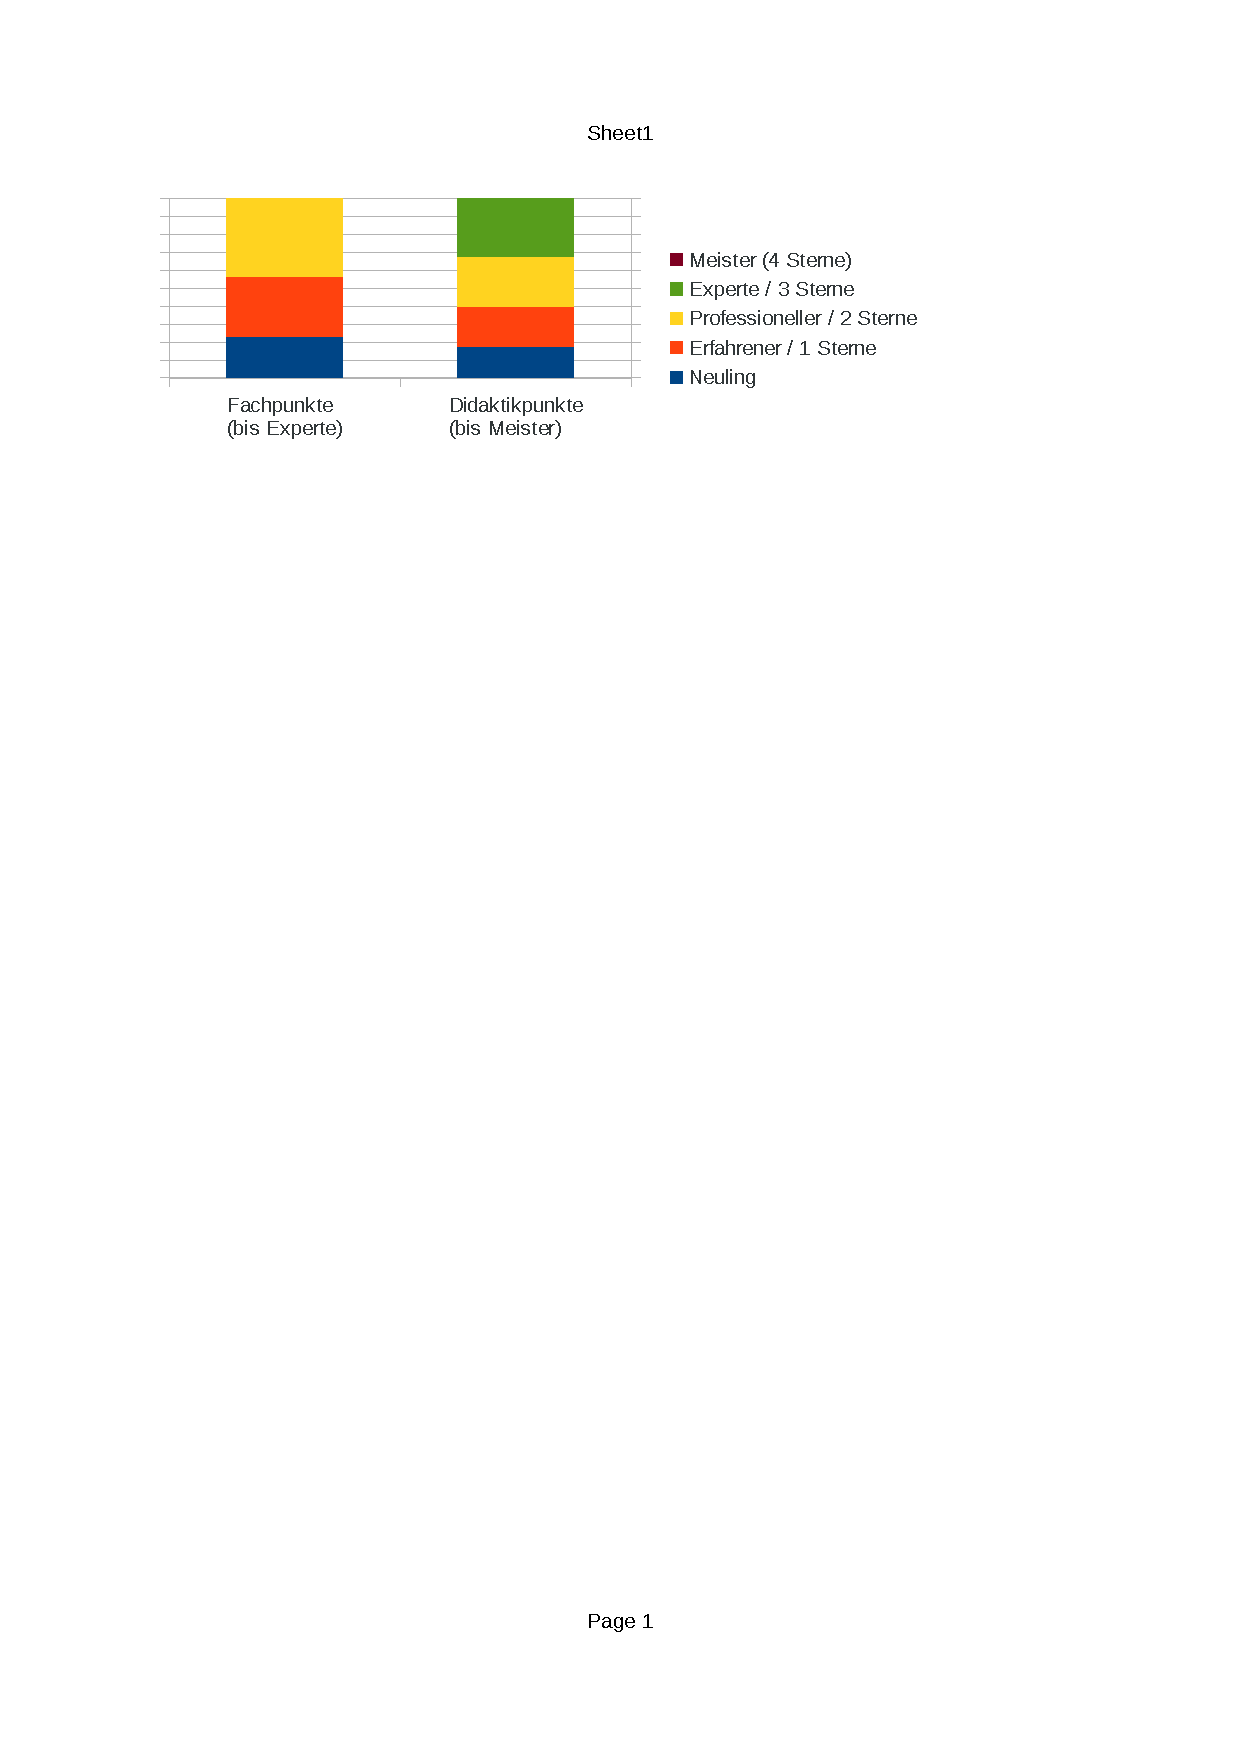
\includegraphics[width=1\textwidth]{verteilungDerPunkte.png}
\caption{Verteilung der Punkte}\label{ref:vertPunkt}
\end{figure}
Ein Meister hat durch das Erhalten der höchsten Wertung für die didaktische
Fähigkeit bereits bewiesen, dass er Spaß an der Vermittlung von Wissen hat.
Demnach bedarf er keiner weiteren Motivation eines höheren Ranges.
Vielmehr möchte er keine negativen Bewertungen seiner Lernenden erhalten und
bemüht sich der weiteren hochwertigen Qualität seiner Lerneinheiten.

\section{Rollen für Anwender}
Passend zum zuvor beschriebenen Konzept werden drei Rollen für Anwender
definiert. Dabei ist das Innehaben mehrerer Rollen zur gleichen Zeit ein Teil
des Modells. Zusammenfassend sind die Rechte und Pflichten eines Nutzers in den
verschieden Rollen in Tabelle \ref{tab:privilegesRoles} aufgeführt. Das dort
aufgeführte Forum ist nicht Teil der ersten produktiven Version (siehe
Abschnitt \ref{ref:weitereIdeen})

\subsection{Administrator}
Der Administrator ist der Verwalter der Plattform und damit für den
reibungslosen Ablauf seitens der Nutzer verantwortlich. Dazu kontrolliert er den
Zusammenhalt des Systems und greift bei inkonsistenzen oder Fehlern ein. Auch
bildet er die Schnittstelle zur Community, die sich in der Weiterentwicklung von
Masterly Mate engagiert.

\subsection{Lernender}
Der Lernende bildet die Hauptzielgruppe des Systems. Er soll WBTs finden, diese
durcharbeiten können und sich an Tutoren wenden, falls er auf ein Problem oder
Unklarheiten stößt. Dazu bietet Masterly Mate ihm das auffinden eines an sein
Fachwissen angepasstes Training. Weiterhin kann er Tutoren kontaktieren, die in
seinem Umkreis wohnen und passend zu seinem Rang Inhalte zu erläutern verstehen.
Die Lokation wird anhand der Postleitzahl festgemacht.

Ein Lernender kann in seinem fachlichen Level bis zum Experten aufsteigen.
Nähere Erläuterungen zu den fachlichen Rängen wurden in Abschnitt
\ref{ref:rankTopic} aufgeführt.

\subsection{Tutor}
Ein Lernender kann ab dem zweiten fachlichen Rang des Dreyfus-Modells (siehe
\ref{ref:dreyfus}) in seinem Profil die Einstellung "`Tutor"' anwählen. Damit
erscheint er unter den Suchergebnissen für Lernende, die einen Tutor suchen. Als
Tutor wird man von Lernenden gefunden, die Unterstützung in einem Fachgebiet
suchen.

\section{Dokumentation der API}\label{ref:archDoc}
RoR bietet ein Werkzeug, welches automatisch eine API-Dokumentation der
Anwendung erstellt. Mit der Kommandozeile \textit{rake doc:app} wird dies
realisiert. Dabei ruft rake\footnote{Kurzwort für Ruby Make} im Namespace doc:
die Funktion app auf, die neben guides und rails die Dokumentation für die
eigene Applikation erstellt. Dabei werden die Kommentare
aus dem Quelltext verwendet, um eine übersichliche Darstellung der
programmierten Funktionen zu schaffen \cite{edgeGuide:2013}.

\section{Automatisch generierte Filterung von Ergebnissen}\label{ref:autoResult}
Die Suche von WBTs wird Über reine SQL-Abfragen realisiert.
Dies bedeutet, dass bei einem Aufruf der WBT-Liste, die Daten des betreffenden
Users ausgelesen werden. Entsprechend des Levels eines Users im betreffenden
Themengebiet werden die Dafür vorgesehenen WBTs, welche er noch nicht
absolviert hat angezeigt.

Alternativ können alle WBTs angezeigt werden, wobei sie nach Themen gefiltert
werden. Bei der Suche wird im Profil des Users nach den dort hinterlegten Themen
gefragt. Im Standardfall werden die Themen die dort aufgelistet sind für die
Suche verwendet. So erhält ein Benutzer mit dem Thema "`Kulturgeschichte des
Buntbarsches und seiner besonderen Bedeutung in der Deutschen Küche"' in
diesem Falle nur WBTs aus diesem Thema. Da jedoch die wenigsten Benutzer bereits
zu beginn ein Thema haben werden, ist es auch möglich alle Themen mit ihren WBTs
anzuzeigen. Der Benutzer kann dann frei wählen, in welchem Thema er sich
weiterbilden möchte. Durch diese vorgehensweise bei der Suche ist die Verwendung
von Suchfeldern und aufwändigen Suchalgorithmen nicht notwendig. Da SQL ohnehin
für die Abfrage von Daten geschaffen wurde ist diese Vorgehensweise außerdem
Performanter als die meisten Suchalgorithmen, welche die Daten ohnehin erst über
SQL beschaffen müssten.
\newpage
\section{Themen}
Die Themen (oder Topics/Themengebiete) grenzen die WBTs voneinander ab und sind
neben den Leveln ein Suchkriterium. Jedes WBT ist Teil mindestens eines
Themengebietes. Außerdem sind die Ränge an die Themen gebunden. Der Benutzer
kann WBTs in jedem Themengebiet absolvieren und im Rang aufsteigen. Dabei ist zu
beachten, dass ein Benutzer einen bestimmten Rang nur in einem Themengebiet
haben kann. Das bedeutet, dass er zwar in einem Gebiet den Status eines
Expertise haben kann, in einem ganz anderen jedoch ein absoluter Newbie ist. Ist
ein WBTs zwei (oder mehr) Themen zugeordnet, so erhält der Benutzer bei
Abschluss die Punkte für beide Themengebiete. 

Themen können Unterthemen haben, daher kann ein Benutzer innerhalb eines
Überthemas unterschiedliche Ränge haben. So kann z.B. ein Benutzer im Thema
Informatik ein Expertise sein und zugleich in den Unterthemen Datenstrukturen
und Algorithmen Advanced bzw. Newbie sein.

Die Beziehung von Benutzer zu Themengebiet ist m:n, ebenso ist die Beziehung
zwischen Thema und WBT m:n. Die Beziehung von Themen zu ihren Unterthemen ist
1:n. 

Das hier Beschriebene ist der Stand der Alpha-Version. Nicht verwendet wurde die
Möglichkeit, Ränge nur in in einem Thema ohne Überthema zu besitzen zu können
und damit Unterthemen hierfür zu sperren. Dies wurde außer acht gelassen, da es
ein höherer Entwicklungsaufwand wäre. Obendrein sind wir zu der Ansicht
gekommen, dass dies nicht dazu führt den Fortschritt eines Benutzers besser
bewerten zu können. So wäre er möglicherweise durch ein einziges Unterthema zum
Expertise in einem Überthema geworden ohne jedoch viele andere Teilaspekte zu
beherrschen. Er wäre damit zwar in dem kleinen Bereich innerhalb des großen
Themas sehr bewandert. Ein breites Wissen, welches seinen Rang in dem großen
Thema rechtfertigen würde hat er jedoch nicht.

Eine weitere Möglichkeit, die außer acht gelassen wurde ist das kaskadieren der
Punkte, welche in einem Unterthema erworben wurden. Dies ist zwar eine recht
gute Näherung an die Realtität allerdings kann auch hier sehr leicht der Fall
auftreten, welcher oben bereits beschrieben wurde.

Eine mögliche Änderung für die Zukunft wäre es jedoch, dass erreichte Punkte zu
einem gewissen Teil dem Überthema gutgeschrieben werden. Man könnte z.B.
die, in einem Thema enthaltenen WBTs in relation zu allen WBTs innerhalb eines
Überthemas setzen und daraus einen Satz errechnen wie viel es für das große
Ganze bringt. So würde z.B. ein WBT mit sehr wenigen und/oder sehr leichten WBTs
nur zehn Prozent seiner Punkte dem Überthema gutschreiben.

Um Missverständnissen vorzubeugen sei hier gesagt, das mit "`Übergeben"' oder
"`gutschreiben"' nicht gemeint ist, dass Punkt vom Unterthema abgezogen und dem
Benutzer im Überthema gutgeschrieben werden, sondern das diese dem Benutzer
sozusagen zusätzlich zur Verfügung gestellt werden. Das abziehen von Punkten zu
gunsten eines Überthemas wäre ein weiterer Punkt, welcher in der Zukunft zu
Diskutieren wäre.

Ein weiterer Punkt der beim Entwurf von Masterly Mate aufgeworfen wurde, ist die
Frage nach der Löschung von Überthemen. Aufgrund von Zeitmangel in der ersten
Version wurde die Löschung so geregelt, dass bei einer solchen, die Unterthemen
und WBTs, des zu löschenden Themas in das übergeordnete Thema verschoben werden.
Dies hat den Grund, dass bei einer solchen Aktion lediglich die Verweise auf das
Überthema geändert werden müssen und dies ohne unnötig großen Aufwand möglich
ist. Die weiter oben aufgeworfene Frage nach den WBTs im Root-Thema wurde in
dieser Version nicht gelöst (Es ist daher möglich im Root-Thema Punkte zu
sammeln und zum "`Master of the Universe"' aufzusteigen). Die Alternative nach
welcher eine Löschung eines Überthemas die Löschung aller darin enthaltenen
Inhalte bedeuten wurde, wurde komplett verworfen, da es Probleme mit den
Berechtigungen der Benutzer geben würde, wenn z.B. ein Tutor ein Thema löschen
würde in dem WBTs liegen, welche er nicht erstellt hat. In der Zukunft muss das
Problem mit den WBTs im Root-Thema angegangen werden. Es wäre sinnvoll, WBTs
welche im Root-Thema liegen für die Benutzung zu sperren.